\section{La separación de variables}

Para la ecuación del crecimiento malthusiano utilizamos que la ecuación $\dfrac{\mathrm{d}X}{\mathrm{d}t}=\rho X$ es equivalente a 
$$\int \dfrac{\mathrm{d}X}{X}=\int \rho\mathrm{d}t$$
Esta idea es una técnica estándar para resolver cierta clase de ecuaciones, llamadas de variables separadas, veamos algunos ejemplos antes de dilucidar por qué funciona el truco de la separación de variables.

\begin{ejemplo}
Consideremos la ecuación $\dfrac{\mathrm{d}Y}{\mathrm{d}X}=-\dfrac{X}{Y}$ esta ecuación diferencial es equivalente a la ecuación integral 
$$
\int Y\mathrm{d}Y =-\int X\mathrm{d}X
$$
integrando formalmente tenemos
$$
Y^2+X^2=\xi
$$
para alguna constante no-negativa $\xi$, las soluciones de este problema son círculos de radio $\xi$ .
\begin{figure}[H]
    \centering
    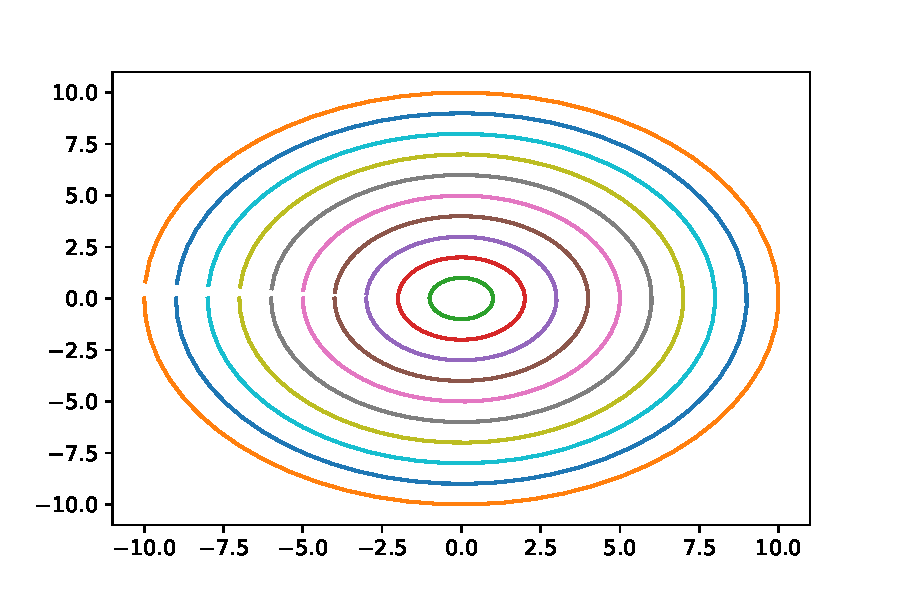
\includegraphics[scale=0.85]{circulos.pdf}
    \caption{Soluciones para el problema $\dfrac{\mathrm{d}Y}{\mathrm{d}X}=-\dfrac{X}{Y}$ }
    \label{fig:circ}
\end{figure}
\end{ejemplo}

\begin{ejemplo}
Consideremos la ecuación $\dfrac{\mathrm{d}Y}{\mathrm{d}X}=\dfrac{Y}{X}$ esta ecuación diferencial es equivalente a la ecuación integral 
$$
\int \dfrac{\mathrm{d}Y}{Y} =-\int \dfrac{\mathrm{d}X}{X}X
$$
integrando formalmente tenemos
$$
\ln(Y)=\ln(X)+\xi
$$
es decir
$$
Y(X)=e^{\xi}X
$$
\begin{figure}[H]
    \centering
    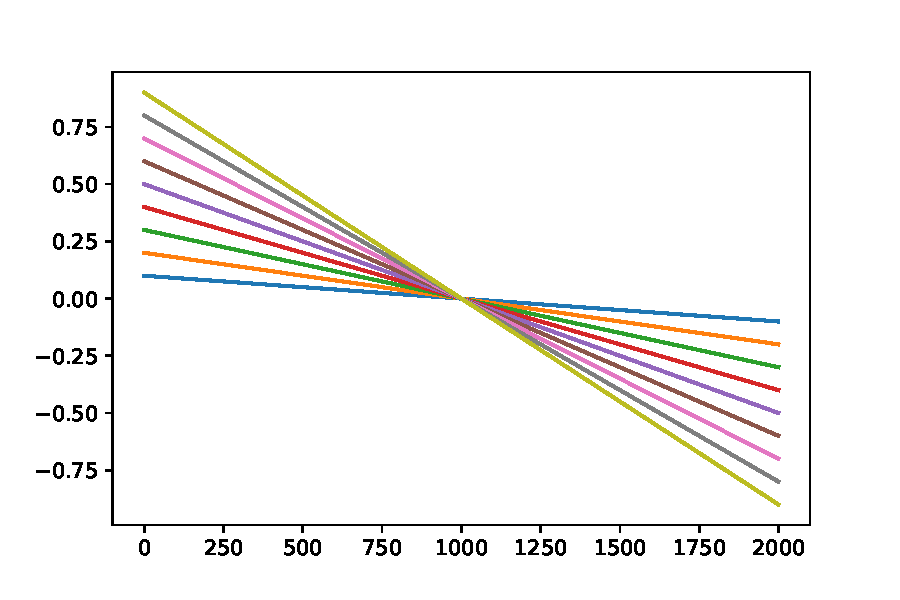
\includegraphics[scale=0.85]{ejemplo2.pdf}
    \caption{Soluciones para el problema $\dfrac{\mathrm{d}Y}{\mathrm{d}X}=\dfrac{Y}{X}$ para distintas condiciones iniciales}
    \label{fig:ej2}
\end{figure}
\end{ejemplo}
 
 Las ecuaciones que están dadas en la forma $\dfrac{\mathrm{d}Y}{\mathrm{d}X}=\dfrac{\Psi(X)}{\Phi(Y)}$ son llamadas de variables separadas, suponiendo que $\Psi$y $\Phi$ son continuas en el dominio correspondiente, entonces la ecuación integral
 $$
 \int\Phi(Y)\mathrm{d}Y=\int\Psi(X)\mathrm{d}X+\xi
 $$
 Esta ecuación integral es llamada finita (¿Se imagina por qué?) y también la satisfacen las soluciones de la ecuación diferencial. Una función de la forma $\Omega(x,y)=0$ que determina a $Y(X)$ como función implícita es llamada integral de la ecuación diferencial, si además esta función determina sin excepción  a todas las soluciones de la ecuación se llama una integral general.
 
 Si $Y(X_0)=Y_0$ es una condición inicial, entonces la integral
 $$
 \int_{Y_0}^{Y}\Phi(Y)\mathrm{d}Y=\int_{X_0}^{X}\Psi(X)\mathrm{d}X
 $$
determina de manera unívoca la solución.

\begin{figure}[H]
    \centering
    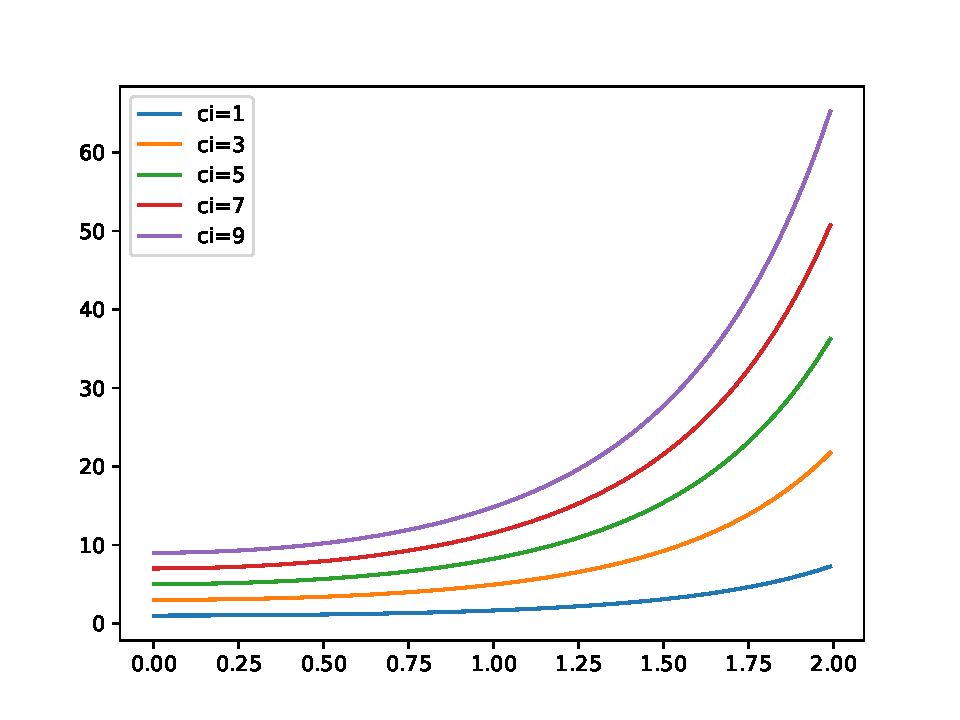
\includegraphics[scale=0.85]{exponenciales1.pdf}
    \caption{Soluciones de la ecuación de Malthus para distintos valores iniciales}
    \label{fig:exposci}
\end{figure}

Dada una condición inicial, para el problema del crecimiento exponencial, hay una solución única, para un valor fijo del parámetro $\rho$, ahora variaremos un poco este parámetro. Tenemos el siguiente comportamiento. 
\begin{enumerate}
    \item Para $\rho=0$ la solución es constante, en general una solución constante es llamada estacionaria.
    \item Para $\rho > 0$ El modelo describe u8n crecimiento ilimitado.
    \item Para $\rho<0$ El modelo describe un decrecimiento asintótico a cero. Podemos representar el cambio cualitativo de las soluciones cuando variamos  el parámetro mediante la llamada linea fase.
\end{enumerate}

\begin{figure}[H]
    \centering
    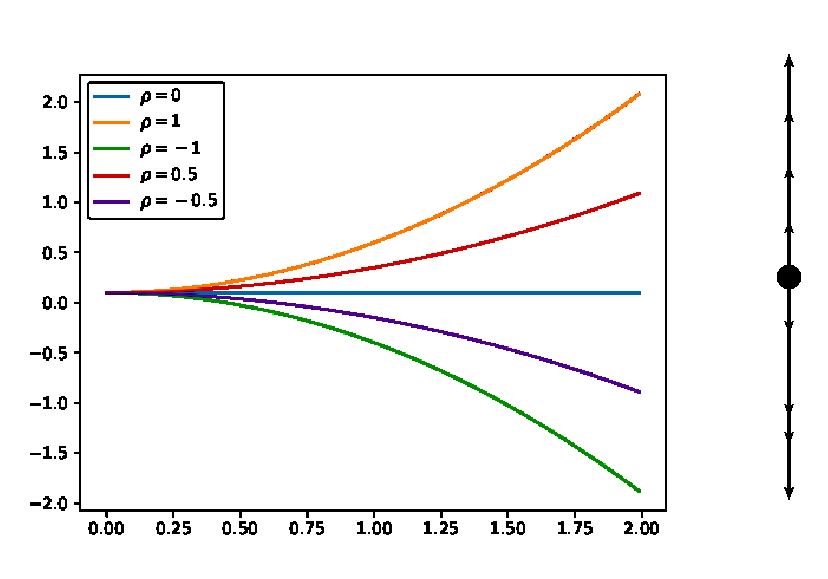
\includegraphics[scale=0.85]{exponenxiales2.pdf}
    \caption{distintos valores para el parámetro $\rho$}
    \label{fig:exposrho}
\end{figure}


Ahora pensemos en la siguiente ecuación:
$$
\varphi_1(x)\psi(y)\mathrm{d}x=\varphi_2(x)\psi_2(y)\mathrm{d}y
$$
no es una de variables separadas. Ahora si tenemos garantizado que : $\varphi_2(x)\neq 0$ y $\psi_2(y)\neq 0$, podemos  considerar la ecuación equivalente
$$
\frac{\varphi_1(x)}{\varphi_2(x)}\mathrm{d}x=\frac{\psi_1(y)}{\psi_2(y)}\mathrm{d}y
$$
que si es de variables separadas. A este tipo de ecuación se le llamda de variables separables.

Ahora hagamos un par de ejemplos sencillos:

\begin{ejemplo}
Consideremos la ecuación

$$
x(1+y^2)\mathrm{d}x-y(1+x^2)\mathrm{d}y=0
$$
está garantizado que  tanto $1+y^2$ como $1+x^2$ son estríctamente positivos, así que nuestra ecuación es equivalente a la ecuación de variables separadas
$$
\frac{y}{1+y^2}\mathrm{d}y=\frac{x}{1+x^2}\mathrm{d}x
$$
que a su vez es equivalente a la ecuación integral
$$
\int \frac{y}{1+y^2}\mathrm{d}y=\int \frac{x}{1+x^2}\mathrm{d}x
$$
cuya solución es 
$$
\ln(1+y^2)-\ln(1+x^2)=\xi
$$
y finalmente, tomando exponencial en ambos términos de la ecuación
$$
\frac{1+y^2}{1+x^2}=e^{\xi}=\zeta
$$
\end{ejemplo}

\begin{ejemplo}
La ecuación
$$
\dot{x}=4t\sqrt{x}
$$
con condición inicial $x(1)=1$ es de variables separables puesto que $\sqrt(x)$ no se anula si empezamos en $1$. Nuestra ecuación es equivalente a:
$$
\frac{\mathrm{d}x}{2\sqrt{x}}=2t\mathrm{d}t
$$
así que
$$
\int_{1}^{x}\frac{\mathrm{d}\xi}{2\sqrt{\xi}}=\int_{1}^{t}2\tau\mathrm{d}\tau
$$
y finalmente
$$
x(t)=t^4
$$
\end{ejemplo}